%===================================================================================
% Chapter: Estado del Arte
%===================================================================================

\chapter{Estado del Arte}
Guerras, incendios forestales, caídas de la bolsa, ataques informáticos, crisis alimentaria, conflictos bélicos, calentamiento global, por solo citar alguno de los problemas que nos atacan en la actualidad. Cada día es más difícil analizar las consecuencias de lo local sin mirar al mundo exterior. En un mundo cada vez más globalizado y a su vez separado en diferentes sectores, clases sociales, religiones u orientaciones políticas; se hace necesario un análisis profundo de la realidad contemporánea para sacar conclusiones objetivas acerca de la cotidianidad, así como, intentar fomentar la toma de decisiones en gobiernos y grandes transnacionales para suavizar o en el mejor de los casos, erradicar ciertas diferencias entre los distintos sectores de la sociedad.

Si existe algo increíble en el mundo que vivimos hoy, es que si bien, somos una sociedad completamente globalizada cada vez vivimos más dispersos en grupos aislados. La globalización esta propiciada en una parte por las increíbles transformaciones en el campo de la informática, las telecomunicaciones y el comercio, unido a la innegable presencia de las potencias mundiales detrás del modelo de pensamiento y la forma de concebir el mundo. ¿Cómo es posible entonces que se explique la existencia de la segregación residencial?

\section{Orígenes de la segregación}

Para poder comenzar un estudio objetivo sobre la segregación residencial se hace necesario resaltar la siguiente pregunta: ¿Qué se entiende por segregación residencial y social? Dicho en términos de White (1983), la segregación en sentido geográfico consiste en la desigual distribución de los grupos sociales en el espacio físico \cite{Rodrguez2008SegregacinRS}. 

Resulta conveniente analizar la existencia de conceptos que refieren a aspectos de ciertos problemas sociales que no son fácilmente separables. Tal es el caso de los conceptos de: “segregación territorial”, “segregación residencial” y “segregación social”. Muchas veces estos conceptos resultan intercambiables. El último de ellos, en disímiles ocasiones se expresa a través de los dos anteriores, sin embargo, no puede ser explicado íntegramente por ellos. “Segregación social”, es un concepto mucho más complejo, y su análisis está marcado por otras variables de lo social que no guardan relación necesaria con el territorio, como pueden ser la situación respecto al mercado de empleo, al acceso a la educación y a los servicios en general. Usualmente hace referencia a las diferencias culturales, normativas, simbólicas y de sensibilidad entre los individuos. “En una sociedad de castas, por ejemplo, la segregación social es virtualmente absoluta, con independencia de la forma en que estas castas se localizan en el territorio; así, en ese caso extremo, la eventual cercanía física de las castas no promovería la interacción entre ellas” \cite{Merkel2014QueEY}.

En la década de los años 20 del pasado siglo, varias disciplinas en el campo de las ciencias sociales mostraron interés por el análisis de los patrones de segregación espacial en las ciudades. La ciudad estadunidense de Chicago fue uno de los epicentros del creciente auge sobre el estudio de dicha problemática. Basándose en analogías de la ecología y la botánica Robert Park presento una representación del mosaico urbano en 1915 \cite{Goist1971CityA}, que tuvo vital importancia en los años venideros. En 1925 E.W. Burgess  presentó un diseño predominantemente concéntrico \cite{Park1984TheCS}. El modelo clásico como luego se conocería la representación de Burgess, describía como los pobres vivían en el centro de la ciudad y los que estaban en mejores condiciones económicas ocupaban los anillos de creciente status social a medida que se alejaban del centro.

\begin{figure}[h!]
	\centering
	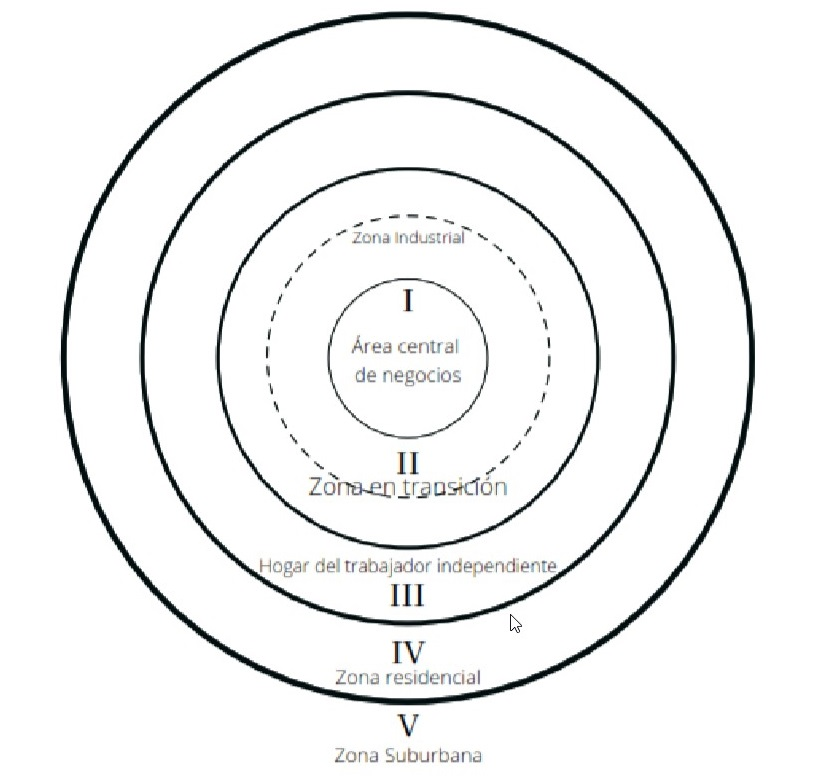
\includegraphics[width=8cm, height=8cm]{Images/Modelo.jpg} 
	\caption{Modelo de Burgues}
\end{figure} 

El modelo clásico se convirtió en un punto de partida para los estudios de segregación, muchas personalidades de la época afines al tema realizaron aportes y contribuciones sobre el mismo. Por un lado, se encontraban las personalidades cuyos ejes de investigación se centraba en los alineamientos topográficos y rutas de comunicación, como fue el caso del sociólogo Homer Hoyt en 1939 \cite{Adams2005HoytH1} y en el otro extremo quienes centraban su atención en el rol de ciertos hitos culturales e históricos como los puntos de anclaje para la élite en los centros de algunas ciudades, como fue: Walter Firey en la ciudad de Boston \cite{Gilmore1947LandUI}.	

A pesar del auge de los estudios de segregación, pareciera que después de abrir el camino hacia el análisis residencial espacial, los sociólogos hubieran perdido su interés en esta cuestión para volver a su tema tradicional orientado a entender el comportamiento de las instituciones sociales y la naturaleza del cambio    social, especialmente como resultado de la urbanización y del impacto del urbanismo como forma   de vida \cite{Manella2014LouisW}. Esto provocó una escasez en cuanto a las publicaciones referentes al tema durante casi una década.
A finales de 1940 se retomaron los estudios enfocados a la medición de la segregación. Uno de los índices que resaltó en estos estudios, sin dudas el más conocido, fue el índice de disimilitud de Duncan \cite{Duncan1955AMA}. El índice de disimilitud representa la proporción del grupo minoritario de una población que tendría que cambiar de residencia para obtener una distribución igualitaria en toda la ciudad. Otros índices surgieron en el transcurso de ese período, pero compartían la limitante de que solo median la segregación en cuanto a dos grupos, lo que refleja el marcado conflicto racial de la época entre personas blancas y negras \cite{Feitosa2004SpatialMO}.
A comienzos de la década de los sesenta se publicó el que para muchos es considerado el libro más influente de la planificación urbana \cite{Jacobs1961TheDA} \cite{NT}. Jane Jacobs, autor del libro, estableció precedentes importantes para el movimiento del Nuevo Urbanismo con respecto a combatir la segregación. Por un lado, defendía la conservación de las diferencias naturales dentro de la ciudad, pero se manifestó en contra de las zonas monopropósito, impulsando en gran medida el desarrollo de las zonas multipropósito que mezclaban trabajo, comercio y residencia. Impulsado principalmente por el modelo desarrollado por Alonso en 1964 \cite{Kirwan1966BookRL}, basado en patrones económico-espaciales para las ciudades, dicha temática pasó a ser de gran interés para los geógrafos. 

\begin{figure}[htb]
	\centering
	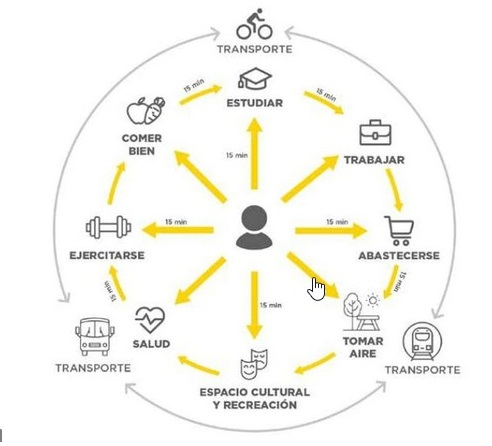
\includegraphics[width=8cm, height=8cm]{Images/ZonaMultiproposito.jpg} 
	\caption{Zonas Multipropósitos}
\end{figure} 

Para finales de los 60 y principio de los 70 los notables avances de las ciencias de la computación, representaron un punto de inflexión en el estudio de la segregación residencial. Los geógrafos contaban con una mayor capacidad para generar “ecologías factoriales” de las ciudades \cite{Clarke1966PopulationPI} \cite{Johnston1978BerryBJ}. Los mapas generados produjeron descripciones bastante matizadas y desagregadas de patrones de distribución espacial de los distintos grupos sociales en las ciudades. Se basaban en correlaciones de análisis factorial de clústeres de variables que parecían estar fuertemente relacionadas.

\begin{figure}[htb]
	\centering
	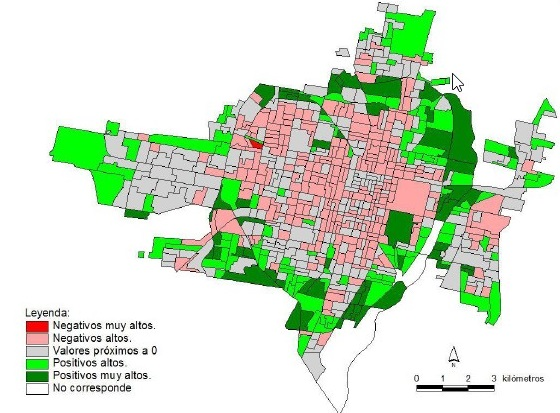
\includegraphics[width=8cm, height=7cm]{Images/EcologiaFactorial.jpg} 
	\caption{Ecología Factorial}
\end{figure} 

Estos clústeres incluían varias características: raza, status socio-económico, edad, por solo citar las más comunes. En efecto estas agrupaciones apuntaban a comprender los procesos subyacentes \cite{Ward1975BrianTR} \cite{Downs1977MapsIM}, pero no lograban explicar realmente por qué la gente elegía determinado lugar para vivir, ni de qué manera se construían sus aspiraciones. En el año 1971 se publicó un artículo pionero en los modelos dinámicos de segregación, el cual si bien en sus inicios estuvo enfocado en el ámbito racial ha tenido una gran trascendencia en todos los estudios de segregación \cite{GoffetteNagot2010IntroducingLC}. Schelling, autor del artículo, propuso un modelo espacial basado en agentes, los cuales cambian su posición acorde a una función de “satisfacción”. Varios son los autores que se basaron en este artículo para trabajos posteriores demostrando la robustez de dicho modelo \cite{Ostolaza2001SobreMD} \cite{Banos2012NetworkEI}. Para finales de los 80, Douglas Massey y Nancy Denton, presentaron un artículo en el cual propusieron cinco dimensiones de segregación: uniformidad, exposición, concentración, centralización y agrupamiento, que pueden ser medidas cuantitativamente a través de índices de segregación \cite{Massey1988TheDO}. Este aporte tuvo gran impacto en los estudios de segregación pues por aquel entonces existía un extenso debate sobre cómo medir correctamente la segregación.

Para los años 2000 los temas vinculados al estudio de la segregación residencial socioeconómica han tenido una presencia constante en los debates académicos y en las agendas públicas de la mayoría de los países del mundo \cite{Luco2003SegregacinRE} \cite{Ham2021}. El basto número de investigaciones referentes a la segregación residencial del pasado siglo y del comienzo de este siglo nos permite afirmar que no es un problema asociado a la sociedad contemporánea, aunque en la actualidad dicha problemática se presenta con mayor visibilidad. Esto se debe a dos fenómenos fundamentales: un primer fenómeno está dado por los estudios recientes que sugieren la existencia un patrón segmentado de localización de los diferentes grupos socioeconómicos en las metrópolis regionales. Un segundo fenómeno es que el mero efecto estadístico, de los asuntos urbanos y metropolitanos han ganado preeminencia entre los problemas de base territorial. Sin embargo, la principal razón por la cual la segregación residencial es un punto más que necesario en la mayoría de las agendas de los debates académicos actuales sobre la sociedad en el mundo, es por las adversidades que la misma trae consigo. 

La visión negativa de la segregación residencial socioeconómica es producto del balance entre facetas contradictorias de la segmentación socioeconómica del espacio. Por una parte, están las desventajas para quienes experimentan dicha segmentación como una forma explícita o disimulada de exclusión y por otra, está el hecho de que para algunos grupos es una opción racional guiada por principios como la maximización de utilidad, la exclusividad, la distinción, la afinidad, la acumulación de activos, la construcción de redes o el acceso a recursos.


\section{Enfoques de los estudios de la segregación} 

La segregación residencial como problema social ha sido altamente estudiada. Siendo abordada por varias disciplinas como son: la sociología, la geografía, la historia y la economía, por solo nombrar las más relevantes. Sin embargo, vale destacar que dependiendo de la región y la época del estudio en cuestión los temas de investigación varían bastante. 

En los Estados Unidos se originaron los primeros estudios sobre dicha temática. Al comienzo los análisis se centraron en las diferencias de étnicas y raciales \cite{Feitosa2004SpatialMO}. Esta problemática, conocida y estudiada desde las primeras décadas del siglo pasado, se mantiene vigente hoy en día y siguen los estudios al respecto. En 2006, se realizó un estudio empleando el índice general de disimilitud, sobre varias ciudades de Estados Unidos. El mismo demostró que la raza continúa siendo un factor importante de segregación, haciendo énfasis en la calidad de educación y viviendas \cite{Selmi2005RaceIT}. El centro para servicio público Weldon Cooper de la Universidad de Virginia elaboró un mapa donde se puede ver la distribución geográfica de los distintos grupos raciales en Estados Unidos, a partir de los datos del censo de 2010 \cite{SDC}. El mapa ofrece una visualización de la distribución geográfica, densidad de población y diversidad racial de la población estadounidense en cada vecindario de todo el país y sirve de base para disímiles estudios acerca de la segregación racial en Estados Unidos \cite{WC}.

\begin{figure}[htb]
	\centering
	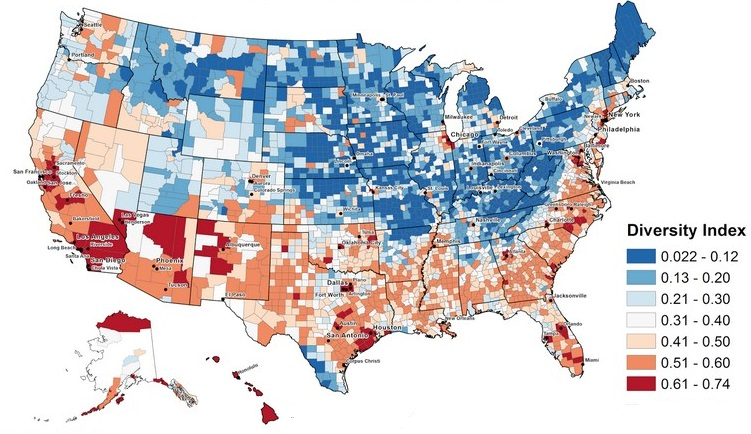
\includegraphics[width=8cm, height=5cm]{Images/WeldomCooper.jpg} 
	\caption{Mapa elaborado por la universidad de Weldon Cooper }
\end{figure} 

Sin embargo, vale destacar que la motivación principal de los estudios acerca de la segregación en los 
Estados Unidos de hoy está asociada a describir otro fenómeno: el claro crecimiento que ha tenido el empleo 
en el área suburbana con respecto al centro de la ciudad. Este creciente desplazamiento de la sociedad americana hacia las zonas no residenciales, resalta la necesidad de estudios de segregación sobre la misma, 
que en palabras de Park y Kwan: “se sabe muy poco sobre la segregación que viven las personas en contextos no 
residenciales“. Un estudio realizado en las ciudades de Atlanta y Georgia utilizó las propuestas de Park y 
Kwan basadas en una nueva noción dinámica de segregación que incluye segregación en varios contextos 
geográficos y temporales en la vida diaria de las personas, lo cual es llamado segregación multi-contexto \cite{Park2018BeyondRS}.


El contexto americano es muy diferente a al contexto europeo, pero los problemas asociados al término: “segregación”, son de igual manera meritorios de estudio. Usualmente el problema de la segregación viene de la mano de otros males sociales como lo son: el crimen, la baja calidad de la enseñanza y las malas condiciones de la vivienda. Los organismos europeos encargados de los estudios de la segregación analizan dicho problema enfocado mayormente a los efectos que ejerce la segregación sobre los vecindarios \cite{Musterd2005HousingMS}. Una problemática que tiene un constante análisis en Europa es la integración de los inmigrantes a la ciudad, tema que es objeto de importantes políticas públicas con distinto grado de éxito \cite{Alonso2008METODOLOGAPE}. Varias son las ciudades que han realizado estudios sobre el tema de la inmigración analizando el problema desde un ámbito más local. 
En el año 2004 se realizó un análisis sobre la población inmigrante de la ciudad de Barcelona \cite{Caas2004IndicadoresCD}. Un artículo publicado en el 2017 \cite{NateraRivas2017EvidenciasSL}, evidenció como la ciudad de Málaga, ha tenido un gran aumento en la afluencia de migrantes desde el 2000, aunque no presenta una segregación residencial extrema, sí indican la existencia de una fuerte precariedad habitacional en los inmigrantes. Un estudio realizado en el 2009 encontró como un fuerte apego a las costumbres y tradiciones étnicas de los inmigrantes da menores posibilidades de empleo \cite{Bisin2009EthnicI}. Sin embargo, el artículo reconoce como las costumbres de los inmigrantes no son fomentadas en sus vecindarios contrariamente a las presunciones que a menudo son expuestas por los medios de comunicación. Un punto importante para analizar la situación de la vivienda de los inmigrantes y por qué viven en espacios segregados, es la discriminación que ejercen las inmobiliarias europeas \cite{Dill2011ResidentialSA}.

\begin{figure}[htb]
	\centering
	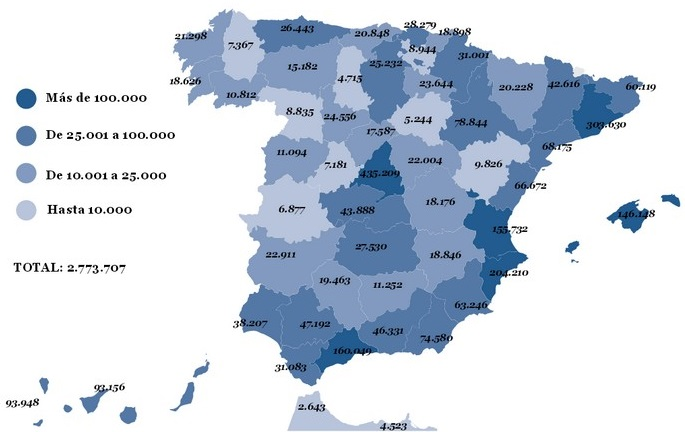
\includegraphics[width=10cm, height=8cm]{Images/Emigrantes.jpg} 
	\caption{Extranjeros de la Unión Europea por provincia en España }
\end{figure}

Por su parte América Latina centra sus estudios en las desigualdades económicas de la población. En la región existe una marcada diferencia entre las condiciones de vida de ricos y pobre en la mayoría de sus ciudades, debido en gran manera a su modelo de ciudad. Los pobres siguen conviviendo en las periferias y los ricos en “conos” de altos ingresos típicamente bien conectados con el centro comercial \cite{Janoschka2002ElNM}. Un estudio realizado en México resaltó como la diferenciación de la población según su condición socioeconómica es uno de los ejes más importantes y críticos de las marcadas diferencias en la sociedad contemporánea, y en particular en la mexicana \cite{Duhau2003DivisinSD}.

Los altos niveles de desigualdad como los que caracterizan a América Latina pueden conducir a la fragmentación de la sociedad como consecuencia del aislamiento de los sectores privilegiados y la exclusión de los más desfavorecidos \cite{Barry1998SocialES}. En este sentido la división social del espacio tiene como componente fundamental la característica de ser la expresión espacial de la estructura de clases o de la estratificación social \cite{Sarav2008MundosAS}. Es decir, si bien existen muchos posibles criterios de diferenciación social que a su vez podrían verse expresados en la estructura espacial, en una sociedad donde cobra una preeminencia absoluta la condición socio-económica para posicionar a los sujetos en la estructura social, esta preeminencia se ve reflejada en el espacio urbano.

De la mano de las marcadas diferencias socio-económicas de américa Latina existe otro problema de gran calibre: “La migración”, ya sea interna o externa. La migración se manifiesta tanto en las zonas de origen como en las zonas de destino, este efecto responde fundamentalmente a la magnitud y, sobre todo, a la selectividad de los flujos migratorios \cite{Vignoli2011MigracinIE}. Estudios realizados reflejan como la afluencia masiva de inmigrantes desde el campo, tiene grandes posibilidades de constituir un vasto sector de población marginada \cite{Elizaga1972MigracionesIE}. Un análisis realizado en varias ciudades importantes de la región, alerta sobre la necesidad de un nuevo enfoque en materia de políticas, sobre todo de las relacionadas con el incremento de la segregación que tiende a provocar la migración \cite{Vignoli2011MigracinIE}.




\subsection{Estudios de la Segregación en Cuba}

Los estudios acerca de la segregación residencial en la isla existen, pero aún son insuficientes. Principalmente orientados a las diferencias socio-económicas en el país y a raíz de la importancia del tema
en los últimos años ha habido un incremento en los estudios sobre el tema. Por su parte, el Centro de
Estudios Demográficos de la Universidad de La Habana (CEDEM) realiza investigaciones sobre cómo afectan las 
diferentes variables demográficas a la estructura poblacional cubana.  

Para entender la segregación social en Cuba y comprender cómo estos males afectan a los habitantes de la isla hay que partir de la base que cuba es un país abrumadoramente urbano. Según el censo del año 2000 el 76 \% de la población cubana era urbana y solo el 40 \% vivía en ciudades de más de 100000 habitantes \cite{CONEI2000}. Lo anterior destaca que un alto porcentaje de la población socializa en contextos urbanos complejos y en una red extendida de medianas ciudades, datos que ciertamente colocan el problema de la regionalización y de la fragmentación urbana en un escenario bastante complicado.

En los años 70 y 80 del pasado siglo la isla con la ayuda del campo socialista fue favorecida por políticas coherentes, basadas en una peculiar situación de recursos de manera abundante. De esta manera Cuba logró evitar en ese entonces alguno de los principales problemas que afrontó América Latina en ese período, como son las desigualdades territoriales extremas y la hipertrofia de las ciudades capitales. El país se organizaba en relación con un sistema de asentamientos humanos que según definió Concepción Álvarez en el año 2001, representaba: “la articulación espacial entre la producción y el consumo” \cite{AC2001}. Este esquema planteaba 4 niveles de asentamientos cada uno con funciones específicas en los esquemas regionales:

\begin{itemize}
	
	\item Una ciudad capital, que operaba con centro proveedor de servicios especializados y cabeza político/burocrática de la isla
	
	\item Una red de trece ciudades intermedias que funcionaban como capitales provinciales, con atribuciones económicas y administrativas sobre su territorio
	\item Un total de 142 ciudades menores (con poblaciones hasta 50000 habitantes), en su mayoría cabeceras municipales, eran proveedoras de servicios sociales y burocráticos.
	\item Una denomina franja base, compuesta por una población dispersa y una miríada de asentamientos urbanos y rurales, donde radicaba el 40 \% de la población de la isla.
	
	
	
\end{itemize}

Gráficamente se trataba de un ordenamiento jerárquico, estructurado desde la capital hasta la población dispersa. Las ciudades intermedias desempeñaban un papel decisivo en la canalización de las inversiones economías. El sistema era abastecido en su tope por los subsidios soviéticos los cuales eran distribuidos hasta la base. Cuba ha cambiado muy poco desde aquellos tiempos, pero la dinámica existente es sustancialmente diferente lo que empuja a una reestructuración espacial.

Tomando esta realidad como punto de partida existen varios análisis acerca situación de la vivienda y la segregación que la misma ha traído consigo, sobre todo en la comparación entorno al año 1959 \cite{Trefftz201150AD} \cite{Pascua2006LasZR}. De la mano de los trabajos que atacan los problemas de la segregación en Cuba de manera general están los que se centran en regiones más específicas. La Habana ha objetivo de varios estudios realizados principalmente enfocados a las diferencias económicas de los habitantes de la ciudad \cite{Herrero2007PlanesDR} \cite{Alfonso2008LaRE}.

\begin{figure}[htb]
	\centering
	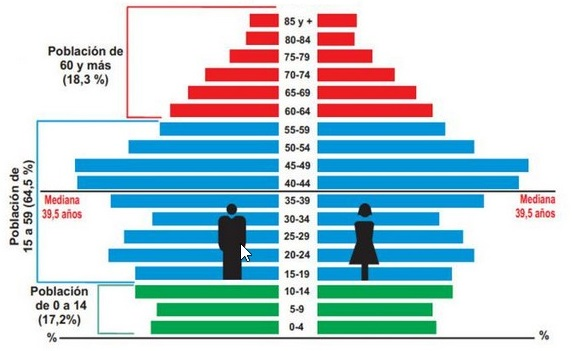
\includegraphics[width=8cm, height=7cm]{Images/CubaEnvejecimiento.jpg} 
	\caption{Estructura de población cubana por sexo y edades .Censo 2012 }
\end{figure}

Una problemática que demanda un análisis urgente en la realidad cubana es el envejecimiento \cite{CONEI2012}. Por una parte, el notable envejecimiento poblacional o demográfico y por otra la antigüedad de las viviendas en Cuba. El envejecimiento poblacional está determinado por disímiles factores: la baja natalidad, la emigración de personas jóvenes, y la elevada esperanza de vida en la isla \cite{Hernndez2015EnvejecimientoPE}. Como este fenómeno impacta directamente en la economía, ya que expresa una disminución en la fuerza laboral, ha sido ampliamente abordado en Cuba \cite{Prez2017ElED} \cite{R2020}. Sin embargo, la problemática del envejecimiento del casco urbanístico y rural cubano es mucho menos abordado. En Cuba el 33 \% de las viviendas tiene al menos 40 años, mientras que en ciudades como la Habana la cantidad de viviendas con al menos 40 años asciende al 51 \% de las viviendas. La investigación de este tema se hace particularmente necesaria, ya que el país se está viendo seriamente afectado por el envejecimiento de sus viviendas. El hecho de poder determinar los sectores más afectados por este fenómeno permite tomar decisiones más certeras, ofreciendo una mejor solución teniendo en cuenta la ubicación geográfica.



\subsubsection{La segregación en la era digital}

Los estudios sobre la segregación residencial en la era digital o de la información, donde todo lo que suene a tecnológico, a inteligencia artificial, a redes sociales se pone a la vanguardia; no pueden negar tales avances. Las nuevas tecnologías para el procesamiento, modelación y almacenamiento de datos proveen herramientas para un análisis más profundo y certero, creando un interés multidisciplinario e interdisciplinario por el análisis de los patrones residenciales y de los procesos sociales. 

El manejo de la llamada Big Data y la inteligencia artificial han permitido el análisis de mayores colecciones de datos \cite{man2018can}. En el año 2011 un artículo propuso la simulación de un modelo multiagente de las dinámicas de una ciudad, en la que sus habitantes cambian su comportamiento en función de las características de su vecindario y de la ciudad en general \cite{Feitosa2011MultiagentSF}. En el 2014, se lanzó una herramienta computacional capaz de 
calcular 43 índices de segregación, con una interfaz sencilla que solo requiere una colección datos geográficos y de población afín a la variable que se quiera analizar \cite{apparicio2014open}. 

En 2018 se realizó una investigación con datos provenientes de la base de datos de red Social Facebook como el sexo, la edad y el lugar de residencia para analizar segregación de género en una zona respecto a la posibilidad de acceso a internet \cite{Fatehkia2018UsingFA}. En la misma se emplearon modelos de correlación para determinar la relación existente entre las variables. Con la utilización de una base de datos geo-codificada y la utilización de modernas herramientas de la inteligencia artificial como la regresión multinomial, en el año 2020 se presentó un artículo que describía un análisis de la segregación residencial en el área de Ámsterdam, teniendo en cuenta salario, población inmigrante, nivel educacional y edad \cite{Boterman2020MultipleDO}. 

Gracias a las ventajas que ofrece la era digital en cuanto a la búsqueda de patrones en el procesamiento de datos, las trayectorias simples \cite{RandonFurling2018FromUS}, aplicadas sobre las ciudades se han convertido en enfoque bastante común en el análisis de la segregación. Las trayectorias simples permiten hacer un análisis multifocal, desde lo local, hasta toda la ciudad. Un estudio desarrollado en el Reino Unido basado en la utilización de trayectorias evidenció como las comunidades cerradas, que se han vuelto populares en las periferias de las ciudades de este país, contribuye y acentúan en gran manera la segregación residencial y alerta de la necesidad de políticas públicas que limite la creación de las mismas \cite{Atkinson2003FortressUG}. Las trayectorias también han sido un pilar fundamental para analizar los movimientos de los inmigrantes y analizar cómo influyen en los vecindarios a los que llegan \cite{Vogiazides2019MigrantsLR}. 

Otro enfoque es la utilización de algoritmos de agrupamiento para detectar si una ciudad o región presenta segregación. Un estudio sobre la ciudad española de Bilbao utilizó K-Means, para determinar la existencia de la segregación de ese territorio \cite{AguadoMoralejo2019AplicacinDU}. El grupo de investigación referente a la inteligencia artificial de la Universidad de la Habana ha realizado varios estudios para analizar la segregación residencial en la Habana tomando como referencia principal el artículo: “From urban segregation to spatial structure detection” \cite{RandonFurling2018FromUS}. Se realizó un trabajo con la utilización de algoritmos de agrupamiento para analiza la segregación respecto a la proporción de casas sociales y el envejecimiento poblacional de la Habana \cite{G2019}.

Estas investigaciones, sobre todo las desarrolladas por el grupo investigativo ge inteligencia artificial de la Universidad de la Habana, relacionadas con trayectorias y algoritmos de agrupamiento constituyen la base teórica para el desarrollo de esta tesis. Los resultados permiten realizar una comparación con los obtenidos en este trabajo.












  
